\begin{center}
	\section{Metodolog\'ia}
\end{center}

\noindent
\justify

En la Figura \ref{metodologia} se muestra la metodolog\'ia empleada para el dise\~no del sistema de eluci\'on y filtrado de la planta de extracci\'on.

% Define block styles: decision, block, line, cloud, blockTwo
\tikzstyle{decision} = [diamond, draw, fill=blue!20, 
       text width=7em, text badly centered, node distance=3cm, inner sep=0pt]
\tikzstyle{block} = [rectangle, draw, fill=blue!20, 
       text width=7em, text centered, rounded corners, minimum height=4em]
\tikzstyle{blockConc} = [rectangle, draw, fill=orange!20, 
       text width=7em, text centered, rounded corners, minimum height=4em]
\tikzstyle{empty} = [rectangle, draw, white, fill=white, 
       text width=-4em, text centered, rounded corners, minimum height=-4em]
\tikzstyle{line} = [draw, -latex']
\tikzstyle{cloud} = [draw, ellipse,fill=red!20, node distance=3cm,
       minimum height=2em]
\tikzstyle{blockTwo} = [rectangle, draw, fill=blue!20, 
       text width=3em, text centered, rounded corners, minimum height=4em]

\begin{figure}[h!]
\centering
\begin{adjustbox}{max width=\textwidth}
\begin{tikzpicture}[scale=1, node distance = 2cm, auto]
       % Place nodes
       \node [block] (init) {Recopilaci\'on de datos};
       \node [cloud, left of=init] (fluid) {Fluido};
       \node [cloud, right of=init, node distance=3.5cm] (part) {Part\'iculas};
       \node [block, below of=init, node distance=3cm] (reco) {Calcular propiedades del fluido};
       \node [block, below of=reco, node distance=3cm] (velsed) {Calcular velocidad m\'axima de sedimentaci\'on $\left(U_{max} \right)$};
       \node [block, below of=velsed, node distance=3cm] (geo) {Definir geometr\'ia de lamelas};
       \node [block, below of=geo, node distance=3cm] (ancho) {Calcular ancho del sedimentador};
       \node [block, below of=ancho, node distance=3cm] (Re) {Calcular $Re$ y $v_0$ en una lamela};
       \node [decision, below of=Re] (ReM) {?`$Re \leq 500$?};
       \node [decision, right of=ReM, node distance=4cm] (velF) {?`$v_0 \geq U_{max}$?};
       \node [empty, left of=ReM, node distance=4.5cm] (red) {};
       \node [block, right of=velF, node distance=4.5cm] (geoI) {Definir geometr\'ia de entrada y tolva de sedimentos};
       \node [block, above of=geoI, node distance=4.5cm] (malla) {Desarrollo CAD y mallado de geometr\'ia};
       \node [decision, above of=malla, node distance=4cm] (check) {Checkeo de malla: ?`es apta?};
       \node [empty, right of=check, node distance=4cm] (remalla) {};
       \node [block, above of=check, node distance=4cm] (cf) {Definir condiciones de frontera};
       \node [block, above of=cf, node distance=4cm] (cfd) {Simulaci\'on CFD};
	   \node [decision, right of=cfd, node distance=4cm] (res) {?`Error mayor al $5 \%$?};
	   \node [block, right of=res, node distance=4cm] (cfdem) {Simulaci\'on CFD-DEM};
	   \node [blockConc, below of=cfdem, node distance=4cm] (conc) {An\'alisis de resultados y conclusiones};     
       
       %\draw (-1.58,-16) -- (-2.5,-16) -- (-2.5, -3) -- (-1.58,-3);
       
       %\node [left of=decide, node distance = 2.5cm] (intermedio)
       % Draw edges
       \path [line] (init) -- (reco);
       \path [line] (reco) -- (velsed);
       \path [line] (velsed) -- (geo);
       \path [line] (geo) -- (ancho);
       \path [line] (ancho) -- (Re);
       \path [line] (Re) -- (ReM);
       \path [line] (ReM) -- node {s\'i} (velF);
       %\path [line] (update) |- (identify);
       \path [line] (ReM) -| node [near start] {no}(red);
       \path [line] (red) |- (geo);
       \path [line] (velF) |- node [near start] {s\'i}(geo);
       \path [line] (velF) -- node {no} (geoI);
       \path [line] (geoI) -- (malla);
       \path [line] (malla) -- (check);
       \path [line] (check) -- node {no} (remalla);
       \path [line] (remalla) |- (malla);
       \path [line] (check) -- node {s\'i} (cf);
       \path [line] (cf) -- (cfd);
       \path [line] (cfd) -- (res);
       \path [line] (res) |- node [near start] {s\'i}(malla);
       \path [line] (res) -- node {no} (cfdem);
       \path [line] (cfdem) -- (conc);
       \path [line,dashed] (fluid) -- (init);
       \path [line,dashed] (part) -- (init);
       %\path [line] (res.west) -- (decide.west);
\end{tikzpicture}
\end{adjustbox}
\caption{Esquema de la metodolog\'ia de dise\~no del presente trabajo.}
\label{metodologia}
\end{figure}

\noindent
\justify

En esta metodolog\'ia se desarrolla el dise\~no del sistema con base en las herramientas anal\'iticas descritas en la secci\'on \ref{simplificado} y al plantemiento num\'erico mostrado en las secciones \ref{DFC} y \ref{MCFDEM}.

\subsection{Recopilaci\'on de datos}

\noindent
\justify

Los criterios de dise\~no del sistema de sedimentaci\'on de placas inclinadas se pueden apreciar en los Cuadros \ref{critSed} y \ref{condiciones}.

\begin{table}[h!]
	\centering
	\begin{tabular}{c|p{4cm}}
		\hline
		\textbf{Par\'ametro} & \textbf{Valor} \\ \hline
		Cantidad de material s\'olido a remover $[kg]$ & 80 \\ \hline
		Densidad media del material s\'olido $\left[kg / m^3 \right]$ & 1700 \\ \hline
		Volumen de la mezcla $[L]$ & 200 \\ \hline
		Tama\~no de part\'icula medio $[\mu m]$ & 250 \\ \hline
		Tipo de solvente & Mezcla agua - etanol ($50 \%$) \\ \hline
		Temperatura del proceso $[\degree C]$ & 28 \\ \hline
		Tiempo del proceso $[h]$ & 1 \\ \hline
	\end{tabular}
	\caption{Condiciones operacionales.}
	\label{condiciones}
\end{table}

\subsection{Propiedades del fluido}

\noindent
\justify

Para desarrollar la automatizaci\'on del dise\~no, es necesario predecir el valor de las propiedades del solvente a cualquier valor de temperatura y relaci\'on agua - etanol. Para ello, se inicia calculando las propiedades del etanol y del agua a presi\'on atmosf\'erica empleando las Ecuaciones \ref{rhoH2O}. \ref{viscH2O}, \ref{rhoEt} y \ref{viscEt}.

\begin{equation}
	\rho _{H_2O} = 1.00048675 \, 10^3 - 2.23243162 \, 10^{-2}*T - 4.60579811 \, 10^{-3}*T^2 \equiv \left[ kg / m^3 \right] 
	\label{rhoH2O}
\end{equation}

\begin{equation}
	\mu _{H_2O} = 1.63190407 \, 10^{-6} - 3.73507082 \, 10^{-8}*T + 3.20602877 \, 10^{-10}*T^2 \equiv \left[ m^2 / s \right] 
	\label{viscH2O}
\end{equation}


\begin{equation}
	\rho _{et} = 8.06320738 \, 10^{2}-8.32481402 \, 10^{-1}*T-5.78205398 \, 10^{-4}*T^2 \equiv \left[ kg / m^3 \right] 
	\label{rhoEt}
\end{equation}

\begin{equation}
	\mu _{et} = 2.11316694 \, 10^{-6} - 3.69955667 \, 10^{-8}*T + 2.57275555 \, 10^{-10}*T^2 \equiv \left[ m^2 / s \right] 
	\label{viscEt}
\end{equation}

\noindent
\justify

Una vez conocidas las propiedades individuales, se calcula la propiedad de la mezcla a trav\'es de la Ecuaci\'on \ref{mezcla}.

\begin{equation}
	\lambda _f = (1-x) \, \lambda _{H_2O} + x \, \lambda _{et}
	\label{mezcla}
\end{equation}

\noindent
\justify

D\'onde: $\lambda$ es la propiedad termodin\'amica (densidad, viscosidad, etc) $x$ es la concentraci\'on de la mezcla.

\subsection{Velocidad m\'axima de sedimentaci\'on}

\noindent
\justify

La velocidad m\'axima de sedimentaci\'on se calcula empleando una metodolog\'ia de c\'alculo iterativa con base en las Ecuaciones \ref{Res}, \ref{CoefArr} y \ref{Uas}. La l\'ogica detra\'s de dicha metodolog\'ia se evidencia en la Figura \ref{UmaxS}.

% Define block styles: decision, block, line, cloud, blockTwo
\tikzstyle{decision} = [diamond, draw, fill=blue!20, 
       text width=7em, text badly centered, node distance=3cm, inner sep=0pt]
\tikzstyle{block} = [rectangle, draw, fill=blue!20, 
       text width=7em, text centered, rounded corners, minimum height=4em]
\tikzstyle{blockConc} = [rectangle, draw, fill=orange!20, 
       text width=7em, text centered, rounded corners, minimum height=4em]
\tikzstyle{empty} = [rectangle, draw, white, fill=white, 
       text width=-4em, text centered, rounded corners, minimum height=-4em]
\tikzstyle{line} = [draw, -latex']
\tikzstyle{cloud} = [draw, ellipse,fill=red!20, node distance=3cm,
       minimum height=2em]
\tikzstyle{blockTwo} = [rectangle, draw, fill=blue!20, 
       text width=3em, text centered, rounded corners, minimum height=4em]

\begin{figure}[h!]
\centering
\begin{adjustbox}{max width=0.53\textwidth}
\begin{tikzpicture}[scale=1, node distance = 2cm, auto]
       % Place nodes
       \node [cloud] (init) {C\'alculo de $U_{max}$};
       \node [block, below of=init, node distance=3cm] (Errac) {Definir criterio de error aceptable: $Err_{ac} \leq 0.01\%$};
       \node [block, below of=Errac, node distance=3cm] (Uas) {Definir un valor inicial de velocidad: $U_{s}=1$};
       \node [block, below of=Uas, node distance=3cm] (Res) {Calcular el n\'umero de Reynolds de la part\'icula $Re_s$};
       \node [block, below of=Res, node distance=3cm] (Carr) {Calcular el coeficiente de arrastre $C$ de la part\'icula};
       \node [block, below of=Carr, node distance=3cm] (Uc) {Calcular la velocidad m\'axima $U_c$ (Ec. \ref{Uas})};
       \node [block, below of=Uc, node distance=3cm] (Errc) {$Err_c = \left| \frac{U_c-U_s}{U_c} \right|$};
       \node [decision, below of=Errc] (comp) {?`$Err_c \leq Err_{ac}$?};
       \node [block, left of=comp, node distance=4.5cm] (Us) {$U_s = U_c$};
       \node [blockConc, right of=comp, node distance=4.5cm] (conc) {$U_{max} = U_s$};
      
       % Draw edges
       \path [line] (init) -- (Errac);
       \path [line] (Errac) -- (Uas);
       \path [line] (Uas) -- (Res);
       \path [line] (Res) -- (Carr);
       \path [line] (Carr) -- (Uc);
       \path [line] (Uc) -- (Errc);
       \path [line] (Errc) -- (comp);
       \path [line] (comp) -- node {no} (Us);
       \path [line] (Us) |- (Res);
       \path [line] (comp) -- node {s\'i} (conc);
\end{tikzpicture}
\end{adjustbox}
\caption{Metodolog\'ia de c\'alculo de la velocidad de sedimentaci\'on m\'axima.}
\label{UmaxS}
\end{figure}

\subsection{Geometr\'ia de lamelas} \label{geoLa}

\noindent
\justify

Se asume una geometr\'ia inicial con base en lo recomendado en el Cuadro \ref{critSed}. La geometr\'ia inicial evaluada es la siguiente:

\begin{table}[h!]
	\centering
	\begin{adjustbox}{max width=\textwidth}
	\begin{tabular}{|c|c|}
		\hline
		\textbf{Par\'ametro} & \textbf{Valor} \\ \hline
		$b [cm]$ & $5$ \\ \hline
		$L/b$ & $8$ \\ \hline
		$\theta [\degree]$ & $60$ \\ \hline
		N\'umero de lamelas & $5$ \\ \hline
		$C_s [m/d]$ & $180$ \\ \hline
	\end{tabular}
	\end{adjustbox}
	\caption{Geometr\'ia inicial supuesta.}
	\label{GeoI}
\end{table}

\subsection{Ancho del sedimentador} \label{anchoSed}

\noindent
\justify

El ancho del sedimentador se calcula con base en la Ecuaci\'on \ref{carS} y a la geometr\'ia inicial mostrada en el Cuadro \ref{GeoI}; definiendo as\'i la geometr\'ia del panel de lamelas del sistema de sedimentaci\'on.

\subsection{C\'alculo de $Re$ y $v_0$} \label{Rev0}

\noindent
\justify

El n\'umero de Reynolds, empleado para evaluar el comportamiento del flujo dentro de la lamela, se calcula con base en lo estipulado en la Ecuaci\'on \ref{Reynolds}. La velocidad media del flujo dentro del sedimentador se calcula con la ayuda de la Ecuaci\'on \ref{v0}.

\subsection{Tuber\'ia de entrada y tolva de sedimentos} \label{enTol}

\noindent
\justify

La tuber\'ia de entrada y tolva de sedimentos se calcula con base en las Ecuaciones \ref{De}, \ref{Des} y \ref{Qdes}.

\subsection{CAD y mallado de geometr\'ia}

\noindent
\justify

Gran parte del \'exito de las simulaciones num\'ericas recaen en la discretizaci\'on del dominio y en la calidad de los elementos que la componen$^{\cite{Roda-Casanova2021}}$. Se desarroll\'o un algoritmo que define la geometr\'ia CAD y realiza el mallado de la geometr\'ia basado en el lenguaje de c\'odigo abierto \texttt{gmsh}. El algoritmo discretiza el dominio con elementos rectangulares (malla estructurada) o triangulares (malla no estructurada). Adem\'as, tiene la capacidad de desarrollar un refinamiento de malla en cada una de las lamelas, como se aprecia en la Figura \ref{malla}.

\subsection{Checkeo de malla}

\noindent
\justify

La evaluaci\'on de la malla se desarrolla con base en el comando \texttt{checkMesh} de OpenFOAM. Los criterios de aprobaci\'on de malla son: \textbf{no ortogonalidad}, \textbf{oblicuidad m\'axima} menor a $1$ y que la \textbf{conclusi\'on} de la malla sea \textbf{ok}.

\subsection{Metodolog\'ia de frontera} \label{CondF}

\noindent
\justify

La mezcla s\'olido-l\'iquida en la entrada presenta un caudal de $0.2 \left[m^3 /h \right]$. La temperatura es constante durante todo el proceso e igual a $28 [\degree C]$. En el tiempo $t=0$, las part\'iculas s\'olidas esf\'ericas se generan en una regi\'on lineal, como se aprecia en la Figura \ref{generation}.

\begin{figure}[h!]
	\begin{tikzpicture}
		\draw (0,0) -- (3,0);
		\draw (3,1) -- (0,1);
		\draw plot [smooth, tension=1] coordinates { (3,0) (3.1,0.25) (3,0.5) (2.9,0.75) (3,1) (3.1,0.75) (3,0.5) };
		
		\draw[red!10!blue, arrows={-Triangle[angle=90:3pt,red!10!blue,fill=red!10!blue]}] (-1,0.5) -- (1,0.5) node [black, text width=2mm] {$\dot{m} _{sol}$};
		
		\draw [dashed, red!50!black] (2.2, -0.2) -- (2.2, 1.2);
		
		\draw[red!30!blue, arrows={-Triangle[angle=90:3pt,red!30!blue,fill=red!30!blue]}] (2.6,0.5) -- (3.4,0.5) node [black, text width=0.5cm] {$\dot{m} _{sol}+\dot{m} _{part}$};
	\end{tikzpicture}
	\caption{Zona de generaci\'on de part\'iculas en la tuber\'ia de entrada.}
	\label{generation}
\end{figure}

\noindent
\justify

De la Figura \ref{generation}: $\dot{m} _{sol}$ se refiere al flujo m\'asico de solvente, $\dot{m} _{part}$ es el flujo m\'asico de part\'iculas generadas y las l\'ineas punteadas representan la zona de generaci\'on.

\noindent
\justify

Las condiciones de frontera se resumen en la Figura \ref{ConFron}.

%Datos geométricos
\def\D{2.7}    	%Diámetro de ingreso
\def\H{3}		%Altura de la zona de lodos
\def\A{2.5}		%Ancho del panel de lamelas
\def\HL{3}		%Altura del panel de lamelas
\def\nL{10}		%Número de lamelas
\def\ang{60}	%Ángulo de inclinación del panel

\def\xlam{\x+\A+0.5*\D}

\def\fin{\nL-1}

%Condiciones de frontera
\def\V{4.44}
\def\P{0}

%Referencia
\def\x{-\A/2-0.5/2*\D-\HL/2}
\def\y{0}

\begin{figure}[h!]
	\centering
	\begin{adjustbox}{max width = 0.5\textwidth}
	\begin{tikzpicture}
		%Geometría general
		\draw (\x,\y) -- (\x,-\D) -- (\x+0.5*\D,-\D) -- 
			(\x+0.5*\D, -2*\D) -- (\x+\A+0.5*\D, -2*\D) -- 
			(\x+\A+0.5*\D, \y) -- ({\xlam + \HL*cos(\ang)},{\y + \HL*sin(\ang)}) -- ({\xlam + \HL*cos(\ang) - \A/\nL}, {\y + \HL*sin(\ang)}) -- (\xlam - \A/\nL, \y) -- cycle;
		
		%Condición entrada
		\draw (\x - 1, \y) -- node[above, rotate=90]  {$\vec{V_0}$} (\x - 1, \y - \D);
		\foreach \yL in {0, ..., 10}
			\draw[red!10!black, arrows={-Triangle[angle=90:3pt,red!10!black,fill=red!10!black]}] (\x-1,\y - \yL*\D/10) -- (\x-0.05,\y - \yL*\D/10);
		
		\draw[red!10!black, arrows={-Triangle[angle=90:3pt,red!10!black,fill=red!10!black]}] (\x,{\y + \HL*sin(\ang)}) -- node[right] {$\vec{g}$} (\x, \y + \H/2);
		%Condición salida		
		\draw ({\xlam + \HL*cos(\ang) - \A/\nL/2}, {\y + \HL*sin(\ang)}) -- ({\xlam + \HL*cos(\ang) - \A/\nL},{\y + \HL*sin(\ang) + \A/10}) -- ({\xlam + \HL*cos(\ang)},{\y + \HL*sin(\ang) + \A/10}) node[above] {$P_0 = P_{atm}$} -- cycle;
	\end{tikzpicture}
	\end{adjustbox}
	\caption{Condiciones de frontera.}
	\label{ConFron}
\end{figure}

\begin{table}[h!]
	\centering
	\begin{tabular}{|c|c|c|}
		\hline
		\textbf{Zona} & \textbf{Propiedad}  & \textbf{Tipo} \\ \hline
		\textit{Entrada} & Velocidad $(V_0)$ & Neumann \\ \hline
		\textit{Salida} & Presi\'on $(P_0)$ & Dirichlet \\ \hline
	\end{tabular}
	\caption{Clasificaci\'on de las condiciones de frontera.}
	\label{CFT}
\end{table}

\noindent
\justify

La clasificaci\'on de las condiciones de frontera se puede apreciar en el Cuadro \ref{CFT}. Al tratarse de una simulaci\'on 2D, las caras frontal y posterior de la geometr\'ia se consideran superficies vac\'ias.

\subsection{Metodolog\'ia CFD} \label{MetCFD}

% Define block styles
\tikzstyle{decision} = [diamond, draw, fill=blue!20, 
       text width=7em, text badly centered, node distance=3cm, inner sep=0pt]
\tikzstyle{block} = [rectangle, draw, fill=blue!20, 
       text width=7em, text centered, rounded corners, minimum height=4em]
\tikzstyle{line} = [draw, -latex']
\tikzstyle{cloud} = [draw, ellipse,fill=red!20, node distance=3cm,
       minimum height=2em]
\tikzstyle{blockTwo} = [rectangle, draw, fill=blue!20, 
       text width=3em, text centered, rounded corners, minimum height=4em]
\tikzstyle{blockConc} = [rectangle, draw, fill=orange!20, 
       text width=7em, text centered, rounded corners, minimum height=4em]

\begin{figure}[h!]
\centering
\begin{adjustbox}{max width = 0.43\textwidth}
\begin{tikzpicture}[node distance = 2cm, auto]
       % Place nodes
       \node [blockTwo] (init) {Inicio};
       \node [cloud, left of=init] (expert) {Datos};
       \node [decision, below of=init] (decide) {?`$t = t_{final}$?};
       \node [blockConc, right of=decide, node distance=4cm] (update) {Fin};
       \node [block, below of=decide, node distance=3cm] (ecu) {$t = t + \Delta t$};
       \node [block, below of=ecu, node distance=2.5cm] (momento) {Resolver ecuaciones de momento};
       \node [block, below of=momento, node distance=2.5cm] (presion) {Resolver ecuaci\'on de presi\'on};
       \node [block, below of=presion, node distance=2.5cm] (vel) {Corregir campo de velocidades};
       \node [block, below of=vel, node distance=2.5cm] (res) {Resolver sistema de ecuaciones};
       
       \draw (-1.58,-16) -- (-2.5,-16) -- (-2.5, -3) -- (-1.58,-3);
       
       %\node [left of=decide, node distance = 2.5cm] (intermedio)
       % Draw edges
       \path [line] (init) -- (decide);
       \path [line] (decide) -- node {s\'i} (update);
       %\path [line] (update) |- (identify);
       \path [line] (decide) -- node {no}(ecu);
       \path [line] (ecu) -- (momento);
       \path [line] (momento) -- (presion);
       \path [line] (presion) -- (vel);
       \path [line] (vel) -- (res);
       \path [line,dashed] (expert) -- (init);
       %\path [line] (res.west) -- (decide.west);
\end{tikzpicture}
\end{adjustbox}
\caption{Solucionador \texttt{pimpleFoam}.}
\label{pimpleLog}
\end{figure}

\noindent
\justify

La simulaci\'on se desarrolla usando el solucionador \texttt{pimpleFOAM}, de OpenFOAM. Desde un punto de vista de \textit{mec\'anica de fluidos computacional}, el problema presenta un flujo con las siguientes caracter\'isticas:

\begin{itemize}
	\item Laminar.
	\item Incompresible.
	\item Transitorio.
	\item Fluido newtoniano.
\end{itemize}

\noindent
\justify

Trat\'andose de un problema bidimensional, \texttt{pimpleFOAM} soluciona la Ecuaci\'on \ref{2D}. La l\'ogica de soluci\'on detr\'as del solucionador se puede apreciar en la Figura \ref{pimpleLog}.


\subsection{C\'alculo del error} \label{errorSimu}

\noindent
\justify

Para la estimaci\'on del error de la simulaci\'on, se emplea la metodolog\'ia descrita en la secci\'on \ref{verified}. Al tener el comportamiento gr\'afico mostrado en la Figura \ref{valsimple}, es posible calcular el error de la simulaci\'on con base en la Ecuaci\'on \ref{errorSimu}.

\begin{equation}
	Err = \left| \frac{\gamma _i - \gamma _{i-1}}{\gamma _i} \right| *100 \leq 5 \%
	\label{errorSimu}
\end{equation}

\noindent
\justify

D\'onde: $Err$ corresponde al porcentaje de error, $\gamma$ a la propiedad de an\'alisis (puede ser velocidad o presi\'on m\'aximas) e $i$ corresponde a la \'ultima iteraci\'on desarrollada con un n\'umero $n$ de nodos definido durante el mallado de la geometr\'ia. El n\'umero de nodos en $i-1$ corresponde a $n/2$.

\subsection{Metodolog\'ia CFD-DEM}

\noindent
\justify

Se emple\'o un solucionador adaptado que vincula OpenFOAM (soluciona las ecuaciones de Navier Stokes) y Yade (soluciona la din\'amica de part\'iculas) a trav\'es de la Interfaz de Paso de Mensajes (MPI, por sus siglas en ingl\'es)$^{\cite{Kunhappan2018}}$. El solucionador emplea el enfoque Euler - Lagrange (ver secci\'on \ref{EuLag}) y \texttt{pimpleFOAM} para predecir la interacci\'on fluido-part\'icula en el tiempo.

\newpage

\noindent
\justify

Para el desarrollo de la simulaci\'on CFD-DEM, se emplearon los datos mostrados en el Cuadro \ref{CFDEMdata}.

\begin{table}[h!]
	\centering
	\begin{adjustbox}{max width = 0.8\textwidth}
	\begin{tabular}{|c|c|}
		\hline
		\textbf{Par\'ametro} & \textbf{Valor} \\ \hline
		\multicolumn{2}{|c|}{\textbf{\textit{Generales}}} \\ \hline
		Material & Arena de r\'io \\ \hline
		Tama\~no de part\'icula $[\mu m]$ & 250 \\ \hline
		M\'odulo de Young & $10 ^6$ \\ \hline
		 N\'umero de part\'iculas por segundo & $22300$ \\
		  \hline
		 $\rho [kg/m^3]$ & 1600 \\ \hline
		 $\nu$ & $0.2$ \\ \hline
		 \multicolumn{2}{|c|}{\textbf{\textit{Coeficientes de par de resorte Dashpot}}} \\ \hline
		 $\alpha$ & $0.12$ \\ \hline
		 $\mu$ & $0.52$ \\ \hline
		 Pasos de resoluci\'on de colisi\'on & 12 \\ \hline
	\end{tabular}
	\end{adjustbox}
	\caption{Datos generales para el desarrollo de la simulaci\'on CFD-DEM.}
	\label{CFDEMdata}
\end{table}

\newpage

\subsection{Software de dise\~no}

\noindent
\justify

Para la ejecuci\'on de la metodolog\'ia mostrada en la Figura \ref{metodologia}, se desarroll\'o un software de dise\~no con herramientas de \textit{c\'odigo abierto}. El software se compone, principalmente, de dos partes: \textit{Frontend} (interfaz de usuario), desarrollada en Jupyter y ParaView, y \textit{Backend} (l\'ogica detr\'as del software), desarrollada en Python, C++ y gmsh. Anexo a este trabajo se encuentran los diferentes componentes desarrollados del software; dando evidencia de la calidad de resultados obtenidos a trav\'es de este.

\subsubsection{Frontend}

\noindent
\justify

La interfaz gr\'afica se desarroll\'o en \textit{Jupyter}. El proyecto Jupyter existe para facilitar el desarrollo de software libre; trat\'andose de un servicio de computaci\'on interactiva que funciona con diferentes lenguajes de programaci\'on, entre ellos: Python y C++. Un ejemplo que permite visualizar el alcance de esta herramienta se puede apreciar en la Figura \ref{jupyter}; en d\'onde se observa la escritura de algoritmos de programaci\'on, evaluaci\'on de la interactividad del algoritmo y documentaci\'on del mismo: todo en una sola pantalla. Jupyter es un acr\'onimo de los lenguajes: \textit{Julia, Python} y \textit{R}.

\begin{figure}[h!]
	\centering
	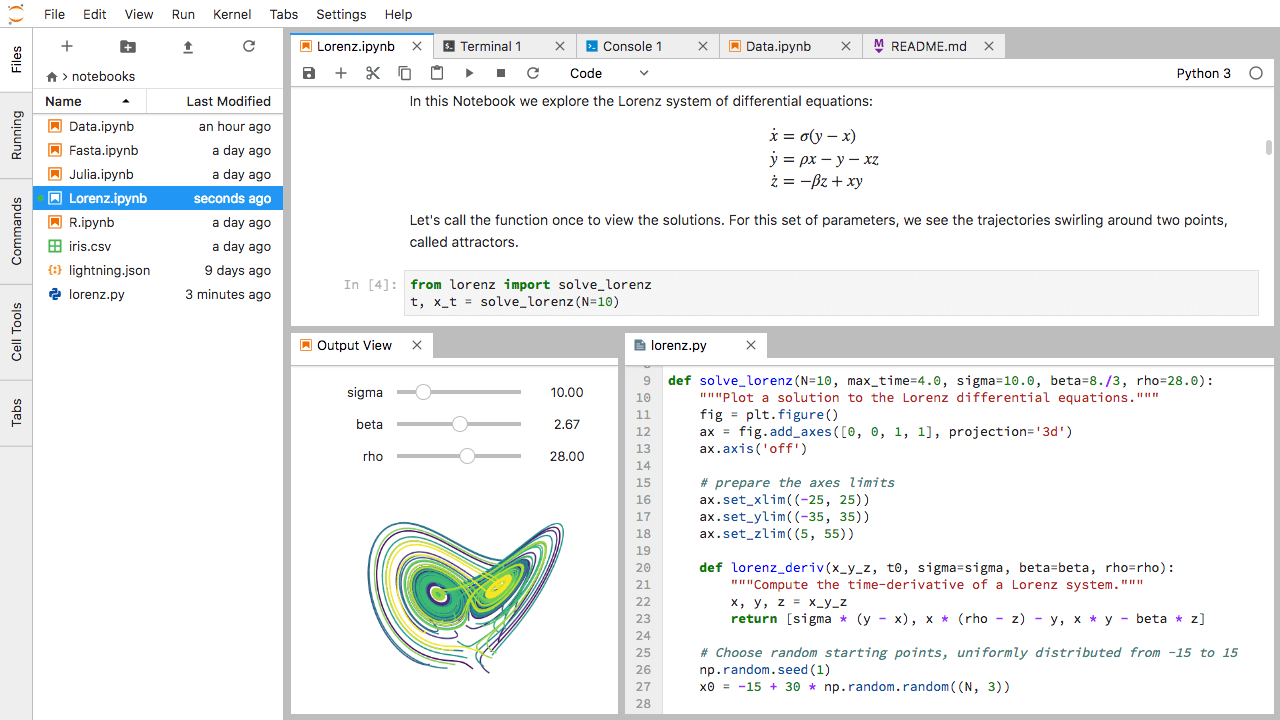
\includegraphics[width=\textwidth]{Images/jupyterlab.png}
	\caption{Interfaz gr\'afica de ejemplo desarrollada con Jupyter. Fuente: https://jupyterlab.readthedocs.io/en/latest/}
	\label{jupyter}
\end{figure}

\noindent
\justify

``Jupyter es una aplicaci\'on web de c\'odigo abierto que permite la creaci\'on y compartibilidad de diferentes documentos, encontr\'andose en ellos: c\'odigo \textit{en vivo}, ecuaciones y visualizaci\'on de texto explicativo. Entre sus usos se encuentran: limpieza y transformaci\'on de datos, simulaciones num\'ericas, modelado estad\'istico y aprendizaje autom\'atico, entre muchos otros." Descripci\'on oficial del proyecto Jupyter.

\noindent
\justify

Parte del Frontend desarrollado para brindar interactividad de usuario se puede apreciar en la Figura \ref{interfaz}.

\begin{figure}[h!]
	\centering
	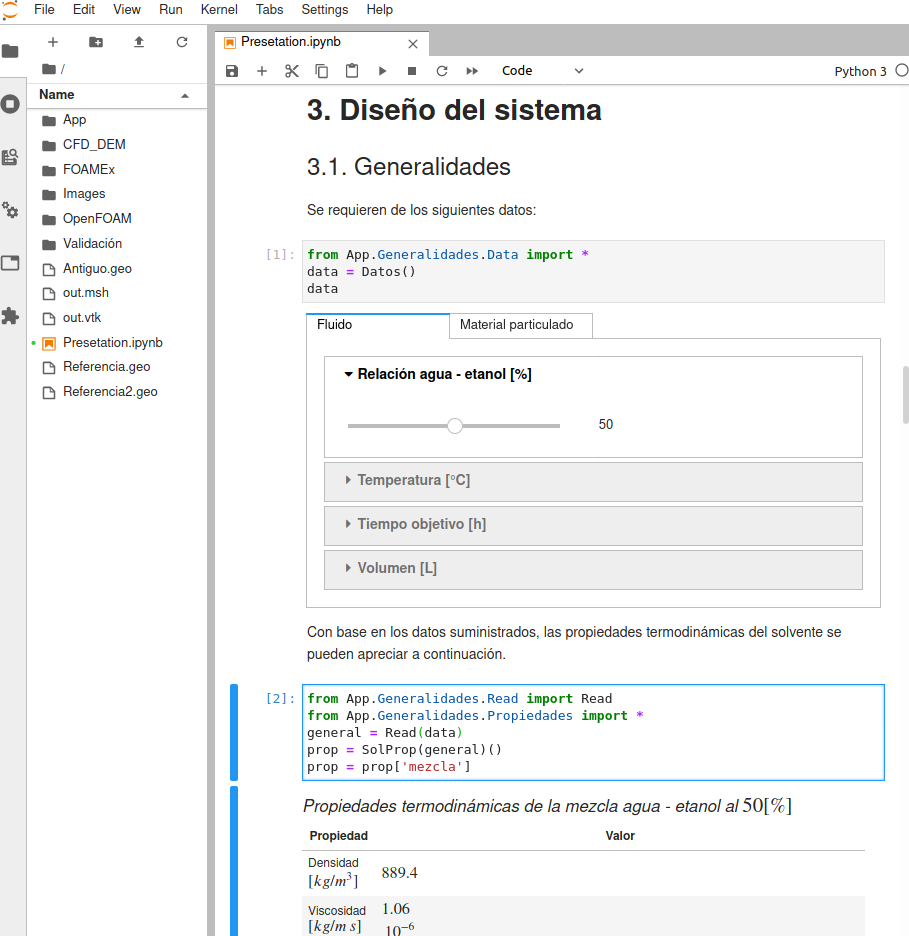
\includegraphics[width=\textwidth]{Images/interfaz.png}
	\caption{Parte de la interfaz gr\'afica desarrollada para la automatizaci\'on del modelo CFD-DEM.}
	\label{interfaz}
\end{figure}

\noindent
\justify


Jupyter permite la interactividad a trav\'es de diferentes lenguajes de Frontend; entre ellos: HTML, CSS y JavaScript. Para la escritura de textos, adopta lenguajes como Markdown y \LaTeX. Adem\'as, cuenta con diferentes librer\'ias internas para el desarrollo de contenidos interactivos, de las que se destacan: \texttt{ipywidgets}, \texttt{IPython.display} y \texttt{Plotly}. 

\begin{figure}[h!]
	\centering
	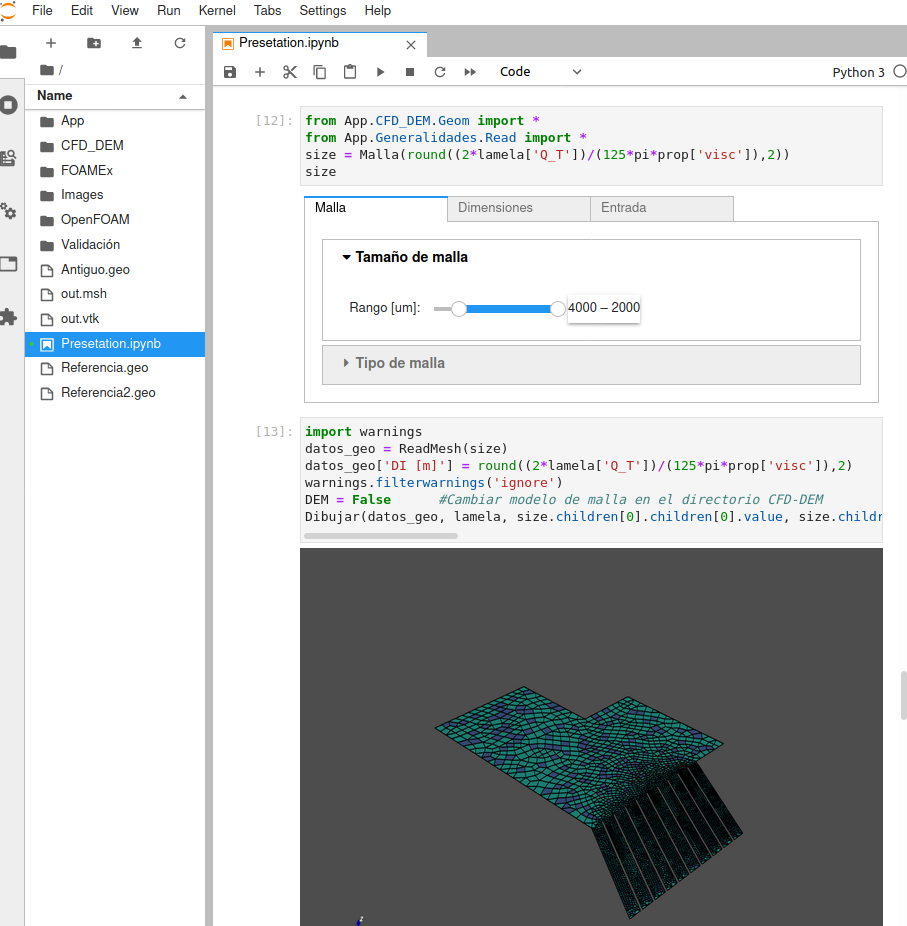
\includegraphics[width=\textwidth]{Images/interfaz2.png}
	\caption{Secci\'on de mallado autom\'atico del software desarrollado mediante \texttt{gmsh}.}
	\label{mallado:gmsh}
\end{figure}

\noindent
\justify

En la Figura \ref{mallado:gmsh} se puede apreciar la interfaz gr\'afica referente al mallado autom\'atico de la geometr\'ia, desarrollado en el lenguaje \texttt{gmsh}; en d\'onde el usuario puede definir el rango de tama\~no de malla, tipo de los elementos (rectangular o triangular) y las dimensiones de la geometr\'ia.

\newpage

\subsubsection{Backend}

\noindent
\justify

Detr\'as de la funcionalidad del software se encuentra el \'arbol de directorios mostrado en la Figura \ref{particion}.

\begin{figure}[h!]
\centering
\begin{forest}
  pic dir tree,
  where level=0{}{% folder icons by default; override using file for file icons
    directory,
  },
  [CFD-DEM Software
    [App
      [{CFD\_DEM}
        [CF.py, file
        ]
        [CFD.py, file
        ]
        [CFDEM.py, file
        ]
        [Geom.py, file
        ]        
        [Malla.py, file
        ]
      ]
      [Generalidades
        [Lamelas.py, file
        ]
        [Propiedades.py, file
        ]
        [Read.py, file
        ]
      ]
      [Sedimentaci\'on
        [Inicial.py, file
        ]      
        [ParOper.py, file
        ]
        [Resultados.py, file
        ]
      ]
    ]
    [{CFD\_DEM}
    ]
    [OpenFOAM
    ]
    [Validaci\'on
    ]
    [Presentation.ipynb, file
    ]
  ]
\end{forest}
\caption{\'Arbol de directorios.}
\label{particion}
\end{figure}

\newpage

\noindent
\justify

El software resuelve, b\'asicamente, tres problemas:

\begin{itemize}
	\item Dise\~no funcional del panel de lamelas desde un enfoque te\'orico.
	\item An\'alisis del comportamiento, a trav\'es de OpenFOAM, de la din\'amica de fluidos del panel de lamelas.
	\item Simulaci\'on CFD-DEM que permite predecir la interacci\'on fluido - part\'icula a distintas condiciones de flujo.
\end{itemize}

\paragraph{Dise\~no funcional te\'orico}

\noindent
\justify

El dise\~no funcional busca defnir una geometr\'ia inicial del panel de lamelas, para el an\'alisis consecuente mediante los m\'etodos num\'ericos de \textit{vol\'umenes finitos} y \textit{elementos discretos}, a trav\'es de metodolog\'ias te\'oricas y experimentales (cap\'itulo \ref{teorico:sed}).

\noindent
\justify

La l\'ogica desarrollada comprende los siguientes pasos:

\begin{enumerate}
	\item Definici\'on, por parte del usuario, de las propiedades del solvente (entre ellas: proporci\'on de la mezcla hidroetan\'olica) y del material particulado.
	\item C\'alculo de las propiedades termodin\'amicas del fluido.
	\item Definici\'on de la geometr\'ia del panel de lamelas.
	\item C\'alculo de las diferentes propiedades del solvente: caudal, velocidad del fluido y de la sedimentaci\'on y el n\'umero de Reynolds, por mencionar algunos.
\end{enumerate}

\noindent
\justify

Los algoritmos que emplean esta l\'ogica se encuentran ubicados en las direcciones \texttt{App/Sedimentaci\'on} y \texttt{App/Generalidades}, como se aprecia en la Figura \ref{particion}.

\paragraph{Simulaciones num\'ericas} \label{imp:CFD}

\noindent
\justify

El modelo CFD permite conocer el comportamiento del solvente dentro del volumen de control para contrastarlo con el modelo CFD-DEM. Comprende los siguientes pasos:

\begin{enumerate}
	\item Definici\'on de la geometr\'ia.
	\item Mallado de la geometr\'ia.
	\item Definici\'on de las condiciones de frontera.
	\item Desarrollo de la simulaci\'on.
	\item Postprocesamiento y presentaci\'on de resultados.
\end{enumerate}

\noindent
\justify

Los algoritmos desarrollados para el desarrollo de este modelo se encuentran ubicados en la direcci\'on \texttt{App/{CFD\_DEM}}:

\begin{itemize}
	\item \texttt{Geom.py} permite establecer la geometr\'ia del problema de acuerdo a los par\'ametros definidos por el usuario.
	\item \texttt{Malla.py} define el mallado de la geometr\'ia, ejecutando el lenguaje \textit{gmsh}.
	\item \texttt{CF.py} define las condiciones de frontera.
	\item \texttt{CFD.py} se encarga de ejecutar la simulaci\'on num\'erica a trav\'es de OpenFOAM.
\end{itemize}

\noindent
\justify

El modelo CFD-DEM predice las interacciones fluido-part\'icula del sistema de sedimentaci\'on. Emplea la misma l\'ogica descrita en la secci\'on \ref{imp:CFD}. La \'unica diferencia radica en la ejecuci\'on del algoritmo descrito en \texttt{CFD.py}; en su lugar, ejecuta el de \texttt{CFDEM.py} que contiene la metodolog\'ia de desarrollo de la simulaci\'on CFD-DEM basada en el m\'etodo Euler - Lagrange.

